\documentclass{beamer}
\mode<presentation> 
\usetheme{CambridgeUS}
\usecolortheme{seagull}
%\setbeamertemplate{headline}
%\setbeamertemplate{footline} 
% To remove the footer line in all slides uncomment this line

%\setbeamertemplate{footline}[page number] 
% To replace the footer line in all slides with a simple slide count uncomment this line

\setbeamertemplate{navigation symbols}{} 
% To remove the navigation symbols from the bottom of all slides uncomment this line

\usepackage{graphicx}
\usepackage{booktabs} 
\usepackage[round]{natbib}
\usepackage{verbatim}
\usepackage{subfigure}
\usepackage{multicol}
\newcommand{\beginbackup}{
	\newcounter{framenumbervorappendix}
	\setcounter{framenumbervorappendix}{\value{framenumber}}
}
\newcommand{\backupend}{
	\addtocounter{framenumbervorappendix}{-\value{framenumber}}
	\addtocounter{framenumber}{\value{framenumbervorappendix}} 
}
%----------------------------------------------------------------------
%	TITLE PAGE
%----------------------------------------------------------------------

\title[Narrative Conservatism]{Narrative Conservatism} % The short title appears at the bottom of every slide, the full title is only on the title page
\author[]{Juan Manuel Garc\'ia Lara, Beatriz Garc\'ia Osma, Fengzhi Zhu} % Your name
\institute[García Lara, Garcia Osma, \& Zhu, 2021] % Your institution as it will appear on the bottom of every slide, may be shorth and to save space
{Universidad Carlos III de Madrid \\ % Your institution for the title page

	\medskip
	\textit{bgosma@emp.uc3m.es}
	\medskip
		\\

\large The University of Manchester

	\medskip} % Your email address
\date{March 10, 2021} % Date, can be changed to a custom date (\today)



\begin{document}
	
\begin{frame}
\titlepage % Print the title page as the first slide
\end{frame}

%-----------------------------------------------------------------
%\begin{frame}
%\frametitle{Outline}
%\tableofcontents
%\end{frame}

%-------------------------------------------------------------------
%	PRESENTATION SLIDES
%----------------------------------------------------
\section{Research Question and Contribution}
%------------------------------------------------

\begin{frame}
\frametitle{Research Question and Contribution (I)}
\begin{itemize}
\item \textbf{Research Question}

\begin{itemize}
\item Is narrative disclosure conservative? \pause
\end{itemize}

\item \textbf{Definition}

\begin{itemize}
	\item Narrative conservatism: narratives that reflect bad news in a \textbf{timelier}, more \textbf{news-consistent}, and \textbf{complete} manner than good news. \pause
\end{itemize}

\item \textbf{Findings}

\begin{itemize}
	\item Using 8-K and 10-Q data (1994-2019), we find evidence of narrative conservatism.
	\item 	Narratives are timelier (shorter time lag), more tone-consistent (content sentiment agrees with sign of news), and have more words, more graphs, more items, and more exhibits in reaction	to bad news than to good news, where news is measured by returns as in Basu (1997).
\end{itemize}
\end{itemize}
\end{frame}


\begin{frame}
\frametitle{Research Question and Contribution (II)}
\begin{itemize}
	\item \textbf{Additional Findings}
	
	\begin{itemize}
		\item Greater narrative conservatism
		\begin{itemize}	
				\item  in voluntary disclosures (compared to mandatory) and MD\&A sections (compared to the notes to financial statements).
				\item in firms with more intangibles and R\&D
				\item where managers have incentives to disclose bad news. \pause
			\end{itemize}		
		\item Pervasive property of narratives in period studied \pause
		\item Greater narrative conservatism in firms with low (high) conditional (unconditional) conservatism
	\end{itemize} \pause
	

	
	\item \textbf{Contribution}
	
	\begin{itemize}
		\item Extend literature on accounting conservatism by defining and documenting the existence of narrative conservatism.
		\item Explore the links between recognition and narrative disclosure.
		\item Add to debate on whether managers withhold bad news. 
		\item Add to literature on narrative properties of SEC filings.
	\end{itemize}
\end{itemize}
\end{frame}
%------------------------------------------------
\section{Theoretical Framework}
%------------------------------------------------
\begin{frame}
\frametitle{Theoretical Framework: Conservatism}
\begin{itemize}
	
	\item \textbf{Accounting Conservatism}
	
	\begin{itemize}
		
		\item Recognition \citep{beaverConditionalUnconditionalConservatism2005,ballEarningsQualityUK2005}
		\begin{itemize}
			\item \textit{Conditional}: ex post or news dependent, ``higher degree of verification to recognize good news as gains than to recognize bad news as losses," \citep*[p. 7]{basuConservatismPrincipleAsymmetric1997} leading to earnings that recognize bad news in a timelier and more complete manner than good news.
			\item \textit{Unconditional}: ex ante or news independent. Aspects of the accounting process (measurement and recognition criteria at the inception of assets and liabilities), leading to a persistent understatement of net assets.
		\end{itemize}
		\pause
		
		\medskip
		
		\item What role narrative disclosure? 
		\begin{itemize}		
			\item  Prior work focuses on recognition, little is known about conservative disclosure \cite[p.243]{kothariManagersWithholdBad2009}.	
			\item A ``committment to timely disclosure of bad news need not come exclusively through financial statement recognition'' \cite*[p. 73-74]{guayConservativeDisclosure2018}:
			
			
		\end{itemize}
		
	\end{itemize}
	
\end{itemize}
\end{frame}
%------------------------------------------------
\begin{frame}
\frametitle{Theoretical Framework: Recognition and Disclosure (I)}
\scriptsize ``\textit{Although financial statements have essentially the same objectives as financial reporting, some useful information is better provided by financial statements and some is better provided, or can only be provided, by notes to financial statements or by supplementary information or other means of financial reporting.}'' (FASB 1984, par.7)  \pause
\medskip

\normalsize
\begin{itemize}
\item \textbf{Reporting requirements (e.g., FASB, IASB)}

\begin{itemize}
	\item \underline{Recognition}: depictions in numbers with captions on the face of the financial statements \citep{schipperRequiredDisclosuresFinancial2007}. \pause
	\item An economic event can be recognized if it satisfies \textit{all}:
	\begin{itemize}
		\item Definition, measurability, relevance, and reliability criteria
		
	\end{itemize}
	
	
	% First, the item must meet the definition of an element of financial statements (definition criterion). Second, the item must have a relevant attribute measurable with sufficient reliability (measurability criterion). Third, the information about the item must be capable of making a difference in user decisions (relevance criterion). Fourth, the information must be representationally faithful, verifiable, and neutral (reliability criterion).
	\pause
	\item Even if criteria are met, annual reports are \textit{still} annual (low frequency and lack of timeliness). Information may need to be disclosed earlier. \pause
	\item \underline{Disclosure}: possibility to \textit{timely} convey information that fails to meet certain recognition criteria
	
	\begin{itemize}
		\item Displays in the notes and supporting schedules that accompany financial statements \citep{schipperRequiredDisclosuresFinancial2007}; but also:		
		\item 10-Qs, 8-Ks, press releases, conference calls, social media, etc.
	\end{itemize}	
	
	
\end{itemize}





\end{itemize}
\end{frame}
%------------------------------------------------
\begin{frame}
\frametitle{Theoretical Framework: Recognition and Disclosure (II)}
\begin{itemize}
\normalsize
\item \textbf{Role of narratives in accounting conservatism} 
\begin{itemize}	
\item Supplement information that cannot be recognized
\item Explain/complement/provide details of recognized line items
\end{itemize}
\pause
\end{itemize}
\begin{block}{\footnotesize 
\textbf{Narrative conservatism}}
Narratives that reflect economic losses (bad news) in a timelier, more news-consistent and complete manner than economic gains (good news).
\end{block}

\pause
\begin{itemize}
\item \textbf{Narratives may \underline{not} be conservative:} 
\begin{itemize}
\item Strategic disclosure and bad news hoarding/smoothing \citep[e.g.,][]{kothariManagersWithholdBad2009,geAcquirersDiscloseGood2011,segalAreManagersStrategic2016,chapmanInformationOverloadDisclosure2019}.
\item ``Full disclosure,'' \citep{guayConservativeDisclosure2018} may imply greater timeliness and completeness of good news disclosure, if all bad news are recognized.
\end{itemize}

\end{itemize}





\end{frame}
%------------------------------------------------


%------------------------------------------------
\begin{frame}
\frametitle{Theoretical Framework: Timeliness}
\begin{itemize}
	\item \textbf{Asymmetric Timeliness}
	
	\begin{itemize}
		\item Timeliness implies that disclosure is made \textit{in time} to be able to influence users' decisions. 
		\item Managers may delay bad news disclosure to mitigate its negative economic consequences \citep{chambersTimelinessReportingStock1984, niessnerStrategicDisclosureTiming2015, segalAreManagersStrategic2016, brockbankStrategicTiming8K2018}.
		\item Managers may accelerate good news disclosure to increase insider profitability  \citep{khalilovAccountingConservatismProfitability2020}.
	\end{itemize}
	
	
	\medskip
	\pause
	\begin{block}{H1a: Asymmetric Timeliness}
		Narrative disclosure is timelier in response to bad news than to good news.
	\end{block}
	
	
\end{itemize}
\end{frame}
%------------------------------------------------
\begin{frame}
\frametitle{Theoretical Framework: Asymmetric News-consistency}
\begin{itemize}
\item \textbf{News-consistency}

\begin{itemize}
\item News-consistency implies that disclosure agrees with the underlying economic event in content sentiment. %Specifically, we interpret it as the degree to which firms use positive tone in narrative disclosure in response to good news and negative tone in response to bad news.
\item Tone influences how information is perceived or processed, and thus it can be employed both to inform or mislead \citep{davisNumbersMeasuringInformation2012, liInformationContentForwardLooking2010, huangToneManagement2014}.
\item Firms may deploy a uniformly positive tone in both good and bad news disclosure, resulting in higher news-consistency in good news disclosure 
\begin{itemize}
\item ``A careful manager might use 90\% positive words in dismissing an employee.'' \citep[p.1206]{loughranTextualAnalysisAccounting2016}
\end{itemize}
\end{itemize}

\medskip
\pause
\begin{block}{H1b: Asymmetric News-Consistency}
Narrative disclosure is more news-consistent in response to bad news than to good news.
\end{block}


\end{itemize}
\end{frame}
%------------------------------------------------
%------------------------------------------------
\begin{frame}
\frametitle{Theoretical Framework: Asymmetric Completeness}
\begin{itemize}
	\item \textbf{Completeness}
	
	\begin{itemize}
		\item Completeness implies that disclosure includes all necessary information for a user to understand the underlying economic event.
		\begin{itemize}
			\item Disclosure reduces information asymmetry: lowers CoC and increases liquidity \citep{diamondDisclosureLiquidityCost1991,diamondOptimalReleaseInformation1985,leuzEconomicConsequencesIncreased2000}
		\end{itemize}
		
		\item Good news disclosure may be completer, relative to bad news, to boost performance \citep{teohEarningsManagementUnderperformance1998, langVoluntaryDisclosureEquity2000}.
		\item Bad news disclosure may be more complete, relative to good news, to avoid litigation risk \citep{skinnerWhyFirmsVoluntarily1994, skinnerEarningsDisclosuresStockholder1997,marinovicNoNewsGood2016}.
	\end{itemize}
	
	\medskip
	\pause
	\begin{block}{H1c: Asymmetric Completeness}
		Narrative disclosure is more complete in response to bad news than to good news.
	\end{block}
	
	
\end{itemize}
\end{frame}
%------------------------------------------------
%\begin{frame}
%	\frametitle{Theoretical Framework: Conservatism Continued}
%	\begin{itemize}
%
%\item \textbf{Is conservatism useful?}
%
%	\begin{itemize}
%		\item Valuation role: provide financial information about the reporting entity that is useful to existing and potential investors, lenders, and other creditors in making decisions about providing resources to the entity \citep[OB2]{fasbConceptualFrameworkFinancial2018b}
%		\item Stewardship role: how efficiently and effectively the entity's management and governing board have discharged their responsibilities to use the entity's economic resources \cite[OB4]{fasbConceptualFrameworkFinancial2018b}
%	\end{itemize}
%
%\item \textbf{Is narrative conservatism useful?}
%	\begin{itemize}
%		\item We posit that narrative conservatism enhances contract efficiency and serves the stewardship role of accounting
%		\item Testable hypotheses to be developed
%	\end{itemize}
%
%\end{itemize}
%\end{frame}
%%------------------------------------------------
\section{Research Design}
%------------------------------------------------
\begin{frame}
\frametitle{Research Design: Proxies}
\begin{itemize}

\item \textbf{Narrative Disclosure Corpora}

	\begin{itemize}
		\item Corpora: 8-K filings because they (a) are more credible, (b) have higher reporting threshold and (c) are more timely than other corporate communication channels.
	\end{itemize}

\item \textbf{Proxies for Textual Properties and News}
	\begin{itemize}
		\item Timeliness: reporting time lag, defined as the number of days elapsed between the news release date and the filing date of the studied disclosure
		\item News-consistency: the marginal change of tone in response to increase (good news) or decrease (bad news) in stock market returns.
		\item Completeness: the total number of 8-K words, filings, items, exhibits and graphs
		\item News: stock returns \citep{basuConservatismPrincipleAsymmetric1997}.
	\end{itemize}

\end{itemize}
\end{frame}
%------------------------------------------------
\begin{frame}
	\frametitle{Research Design: Model}
	\begin{itemize}

\item \textbf{Model Specification}
%	\begin{itemize}
%		\item Form 10-Q
%		
%		\begin{figure}[h]
%			\centering
%			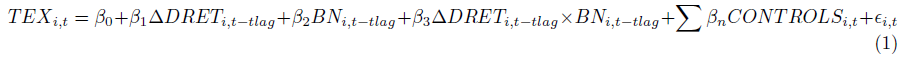
\includegraphics[width=0.75\linewidth]{eq1}
%			\label{eq1}
%		\end{figure}
%	
%		\item Form 8-K
		
		\begin{figure}[h]
			\centering
			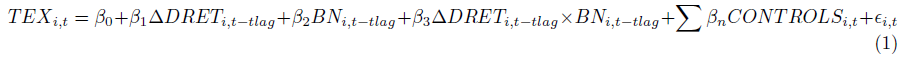
\includegraphics[width=1\linewidth]{eq1}
			\label{eq1}
		\end{figure}
	
		\begin{figure}[h]
			\centering
			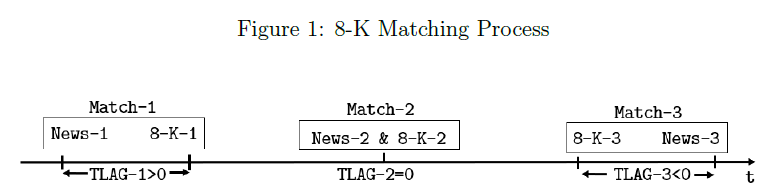
\includegraphics[width=0.8\linewidth]{fig1}
			\label{fig1}
		\end{figure}
%	\end{itemize}

\end{itemize}
\end{frame}
%------------------------------------------------
\begin{frame}
\frametitle{Research Design: Data}

\begin{itemize}
	\item Data source: Compustat, CRSP and I/B/E/S
	
	\begin{figure}[h]
		\centering
		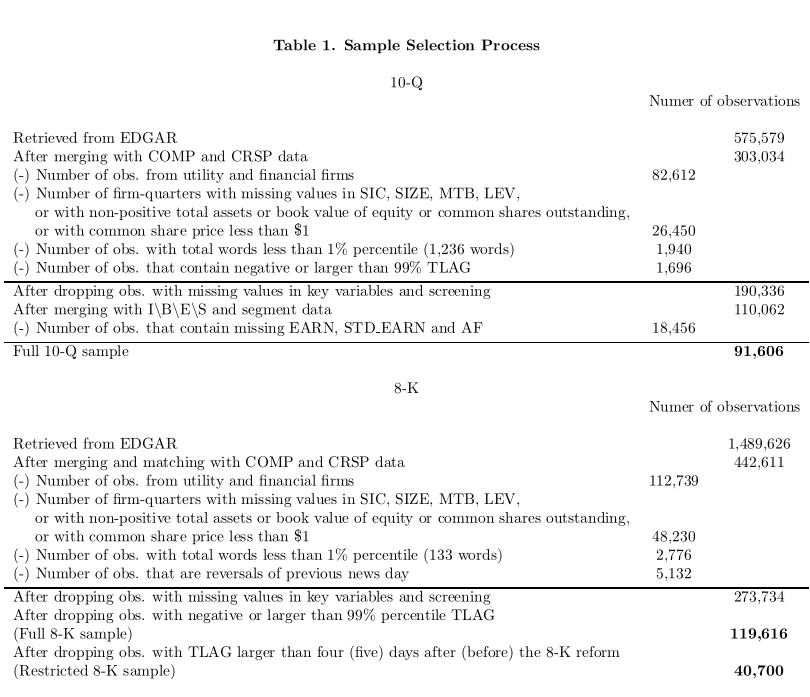
\includegraphics[width=1\linewidth]{tab1}
		\label{tab1}
	\end{figure}

\end{itemize}
\end{frame}
%------------------------------------------------
\section{Results}
%------------------------------------------------
\begin{frame}
\frametitle{Results: Summary Statistics}
\begin{figure}[h]
	\centering
	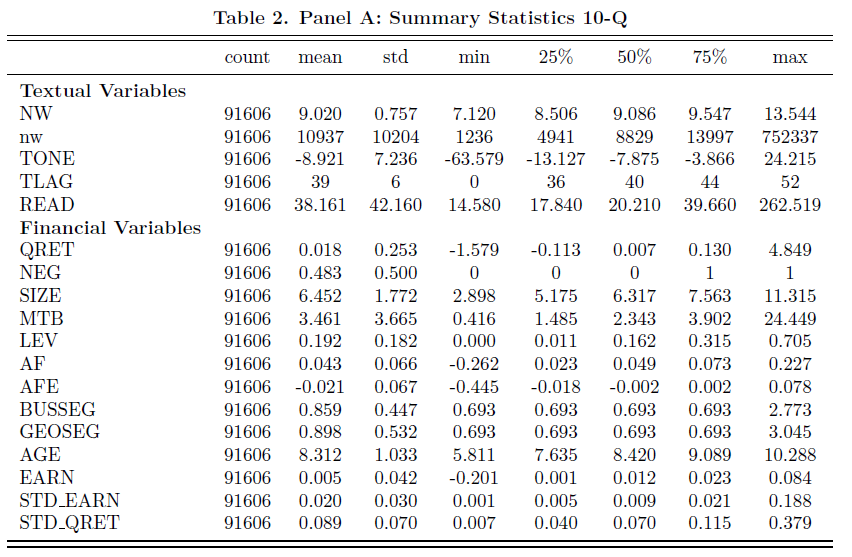
\includegraphics[width=0.65\linewidth]{tab2panA}
	\label{tab2panA}
\end{figure}

\end{frame}
%------------------------------------------------
\begin{frame}
	\frametitle{Results: Summary Statistics Continued}
	\begin{figure}[h]
		\centering
		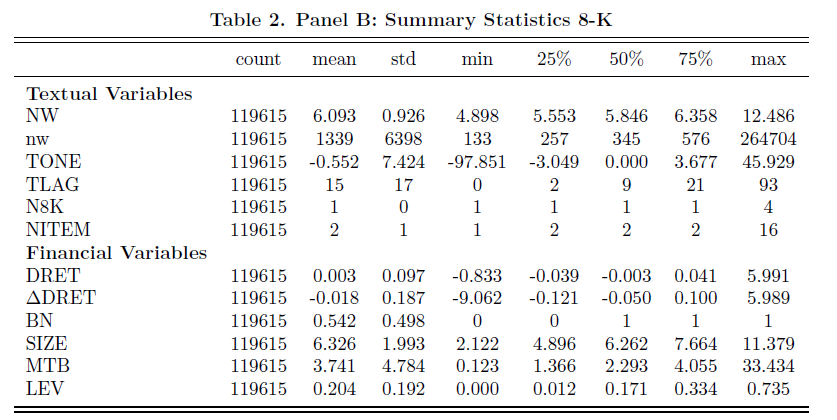
\includegraphics[width=0.55\linewidth]{tab2panB}
		\label{tab2panB}
	\end{figure}
	
\end{frame}
%------------------------------------------------
\begin{frame}
\frametitle{Results: Is 8-K Narrative Disclosure Conservative?}
	\begin{figure}[h]
	\centering
	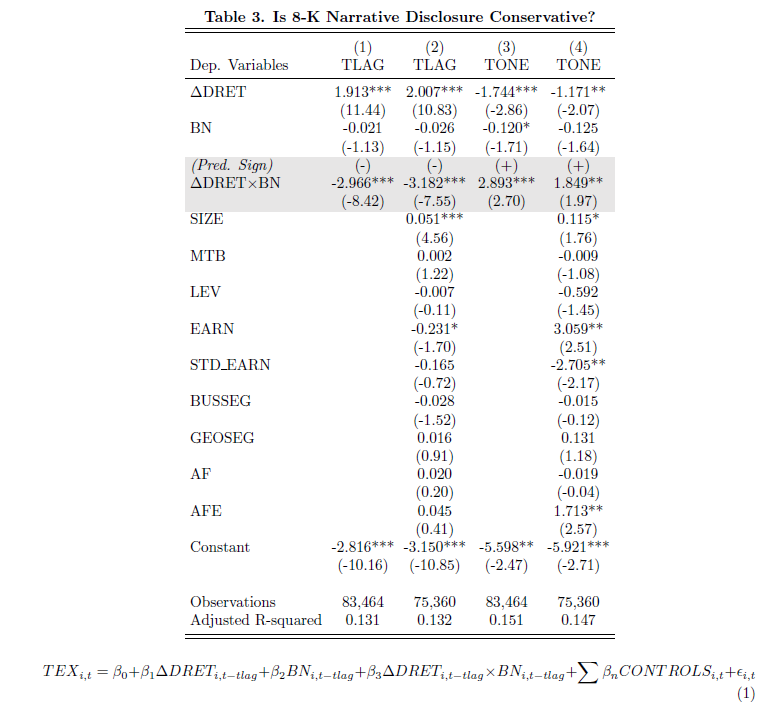
\includegraphics[width=0.7\linewidth]{tab3}
	\label{tab3}
	\end{figure}
\end{frame}
%------------------------------------------------
\begin{frame}
	\frametitle{Results: Is 8-K Narrative Disclosure Conservative?}
	\begin{figure}[h]
		\centering
		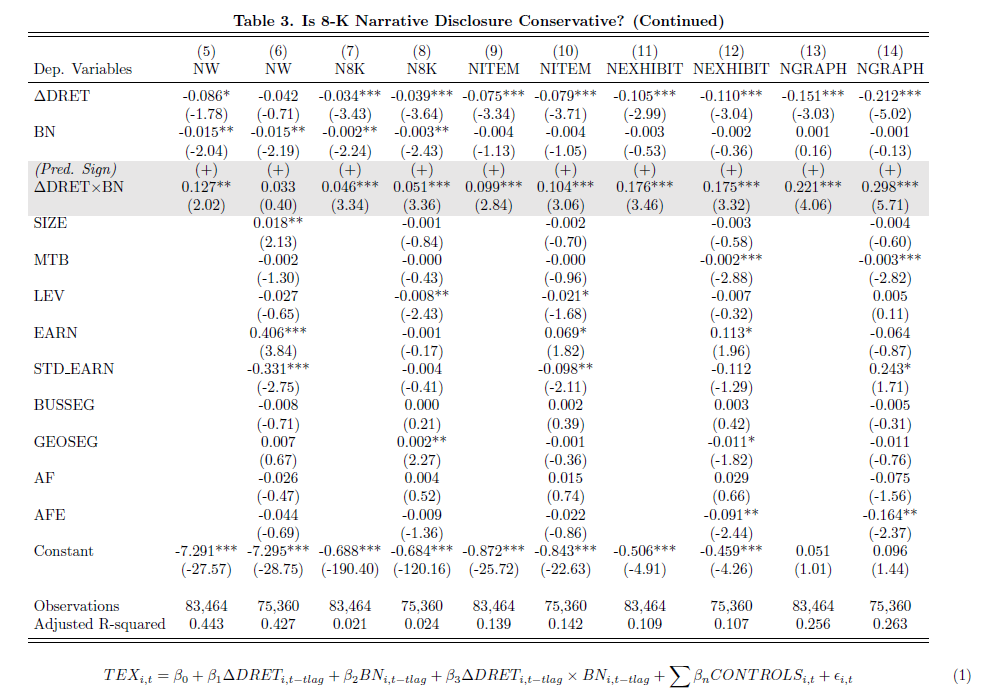
\includegraphics[width=0.8\linewidth]{tab3_cont}
		\label{tab3_cont}
	\end{figure}
\end{frame}
%------------------------------------------------
\begin{frame}
	\frametitle{Results: Robustness Checks}
\begin{itemize}
	\item Our evidence of narrative conservatism is robust to 
	\begin{itemize}
%		\item employing an alternative tone measure using the positive and negative word list from the Harvard General Inquiry dictionary \citep{loughranTextualAnalysisAccounting2016};
%		\item including controls for conditional conservatism and managerial incentives;
		\item excluding 8-K items on results of operations that contain quarterly or annual financial statements \citep{segalAreManagersStrategic2016};
		\item using an alternative 8-K reporting time lag definition \citep{carterRelevanceForm8K1999, niessnerStrategicDisclosureTiming2015, chapmanInformationOverloadDisclosure2019};
		\item excluding a priori bad news 8-K items \citep{segalAreManagersStrategic2016};
	\end{itemize}
\end{itemize}
\end{frame}
%------------------------------------------------
\section{Additional Analyses}
%------------------------------------------------
\begin{frame}
	\frametitle{Additional Analyses: 10-Qs}
	\begin{figure}[h]
		\centering
		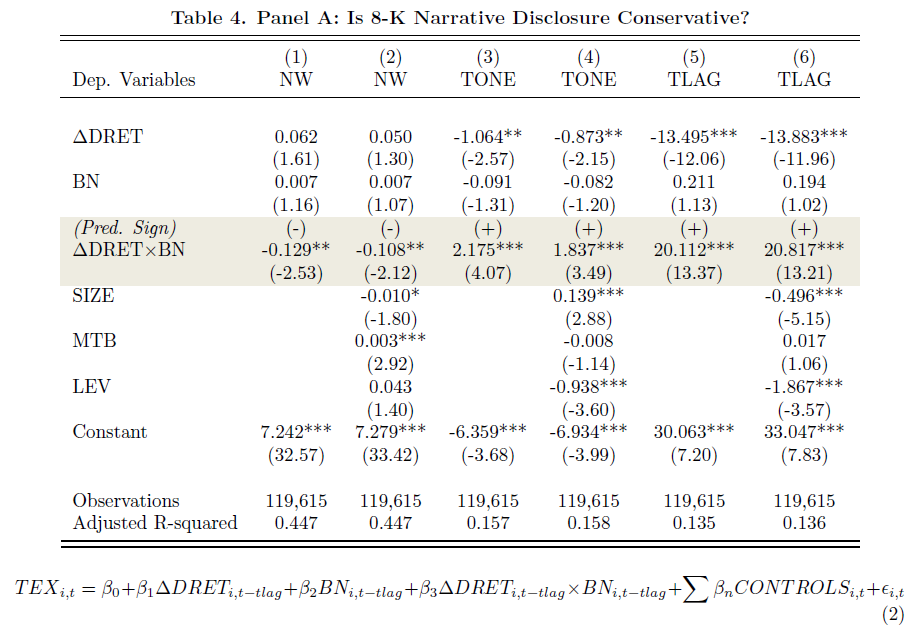
\includegraphics[width=0.6\linewidth]{tab4panA}
		\label{tab4panA}
	\end{figure}
\end{frame}
%------------------------------------------------
\begin{frame}
\frametitle{Additional Analyses: MD\&A and NFS in 10-Qs}
	\begin{figure}[h]
	\centering
	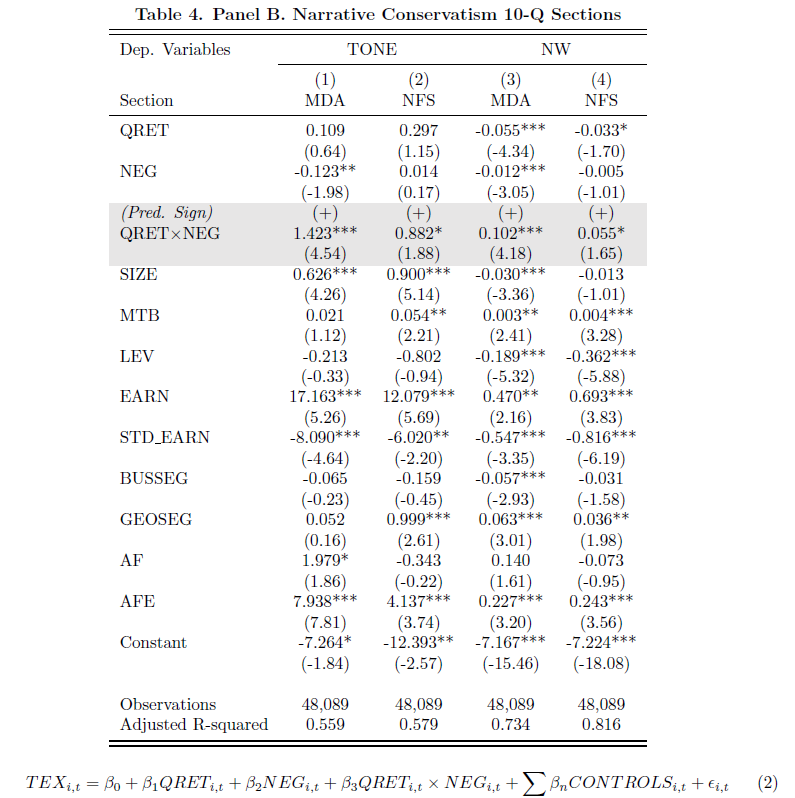
\includegraphics[width=0.58\linewidth]{tab4panB}
	\label{tab4panB}
	\end{figure}
\end{frame}
%------------------------------------------------
\begin{frame}
\frametitle{Additional Analyses: Voluntary and Mandatory Disclosure}
	\begin{figure}[h]
	\centering
	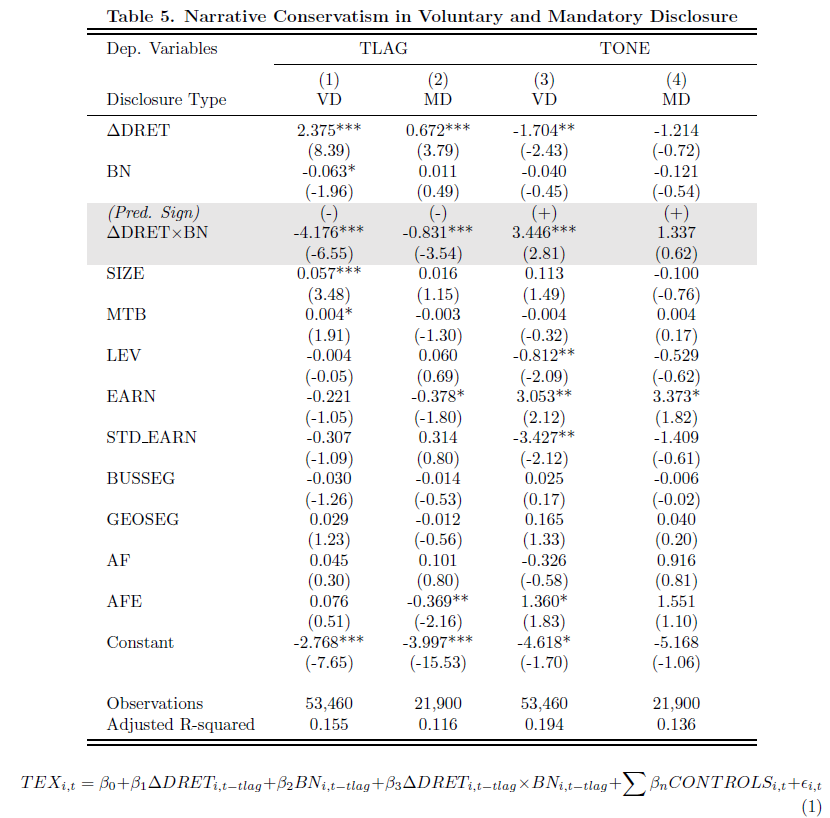
\includegraphics[width=0.63\linewidth]{tab5}
	\label{tab5}
	\end{figure}
	
\end{frame}
%------------------------------------------------
\begin{frame}
	\frametitle{Additional Analyses: Voluntary and Mandatory Disclosure}
	\begin{figure}[h]
		\centering
		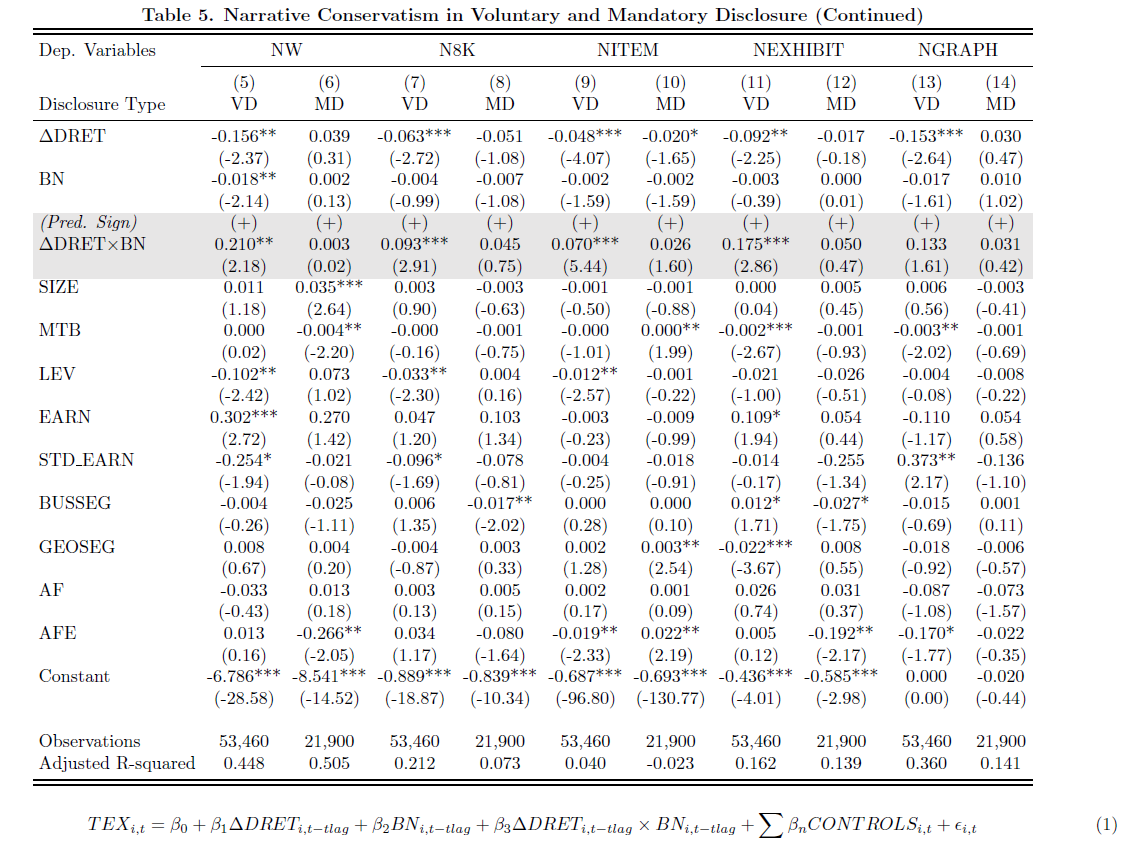
\includegraphics[width=0.8\linewidth]{tab5_cont}
		\label{tab5_cont}
	\end{figure}
	
\end{frame}
%------------------------------------------------
\begin{frame}
	\frametitle{Additional Analyses: Trends in Narrative Conservatism}
	\begin{figure}[h]
		\centering
		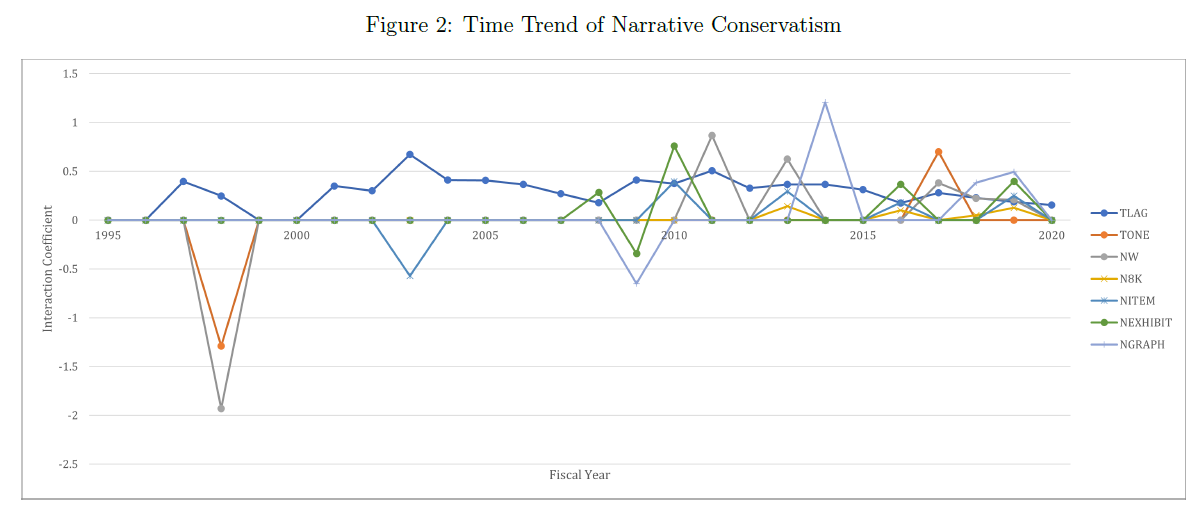
\includegraphics[width=0.9\linewidth]{fig2}
		\label{fig2}
	\end{figure}
	\begin{footnotesize}
		Figure 2 illustrates the time trend of narrative conservatism. X axis represents fiscal year and Y axis represents significant $\beta3$s obtained from yearly
		regressions as specified by Equation (1). Insignificant $\beta3$s are replaced with zero.
	\end{footnotesize}
\end{frame}
%------------------------------------------------
\begin{frame}
	\frametitle{Additional Analyses: Narrative and Conditional Conservatism}
	\begin{figure}[h]
	\centering
	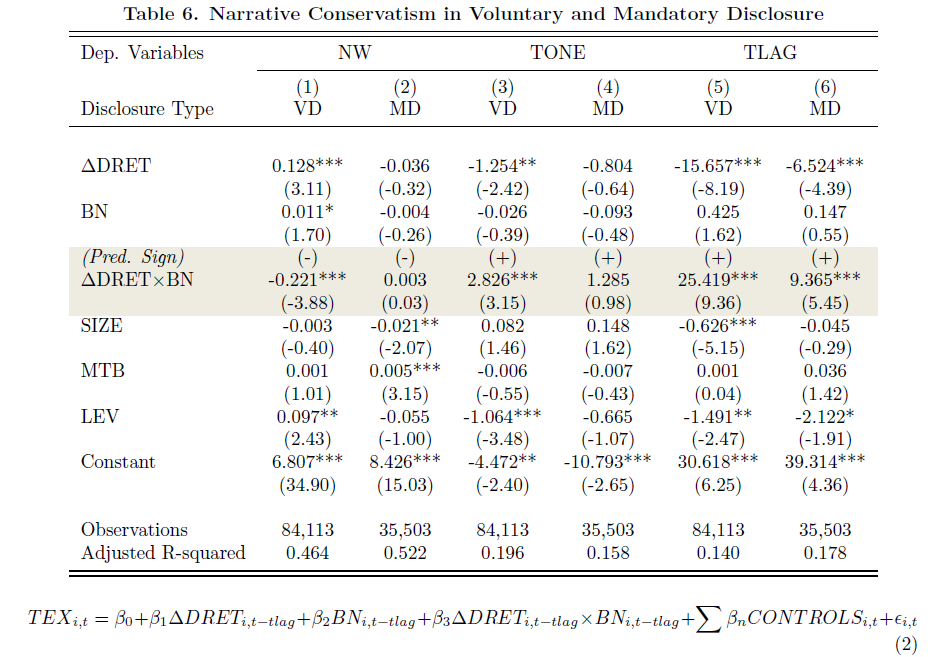
\includegraphics[width=0.6\linewidth]{tab6}
	\label{tab6}
	\end{figure}
	
\end{frame}
%------------------------------------------------
\begin{frame}
	\frametitle{Additional Analyses: Narrative and Conditional Conservatism}
	\begin{figure}[h]
		\centering
		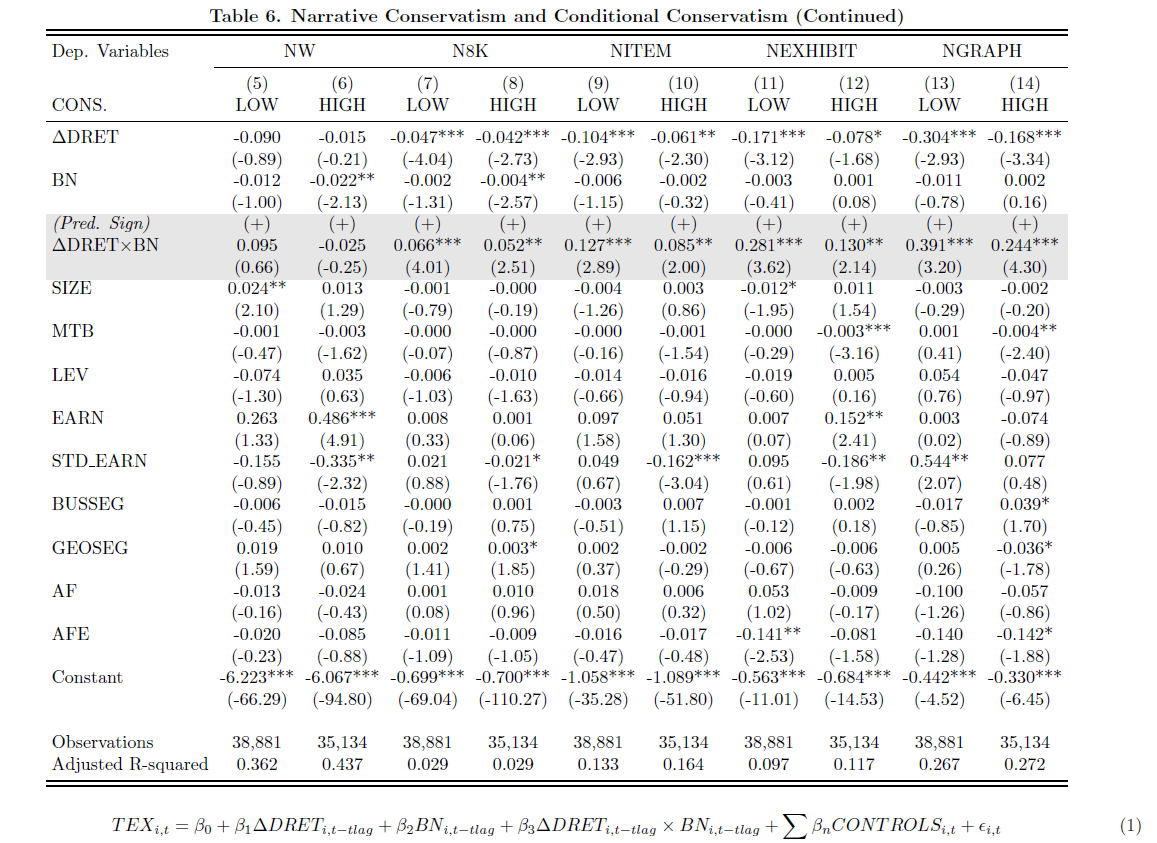
\includegraphics[width=0.8\linewidth]{tab6_cont}
		\label{tab6_cont}
	\end{figure}
	
\end{frame}
%------------------------------------------------
\begin{frame}
	\frametitle{Additional Analyses: Narrative and Unconditional Conservatism}
	\begin{figure}[h]
		\centering
		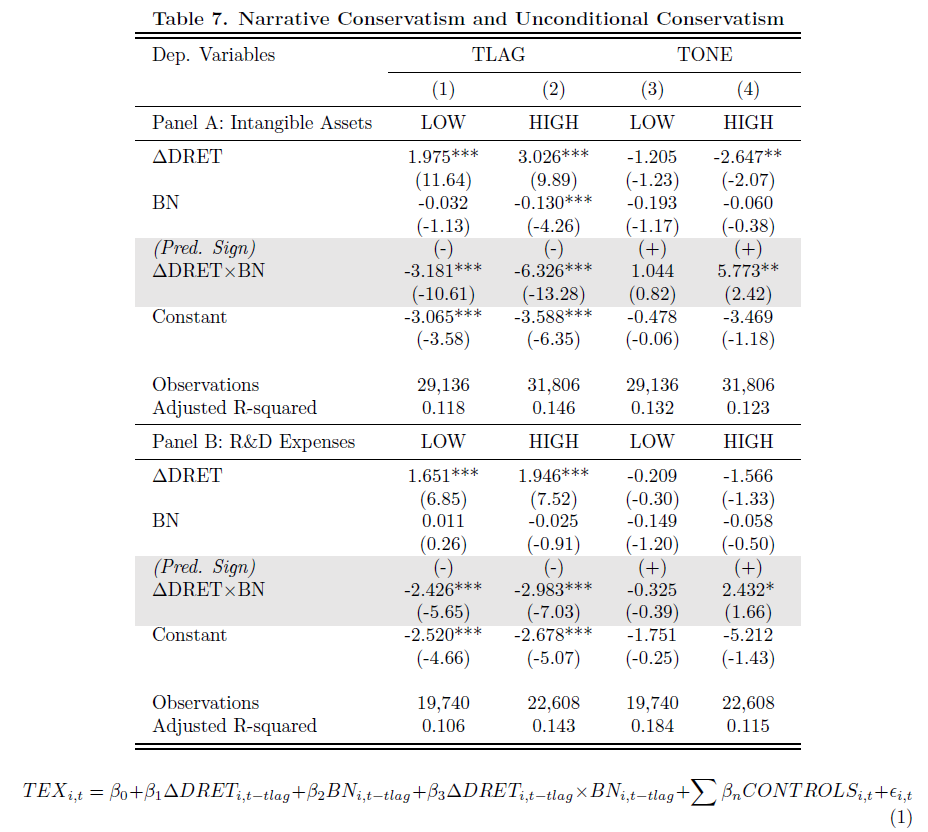
\includegraphics[width=0.6\linewidth]{tab7}
		\label{tab7}
	\end{figure}
	
\end{frame}
%------------------------------------------------
\begin{frame}
	\frametitle{Additional Analyses: Narrative and Unconditional Conservatism}
	\begin{figure}[h]
		\centering
		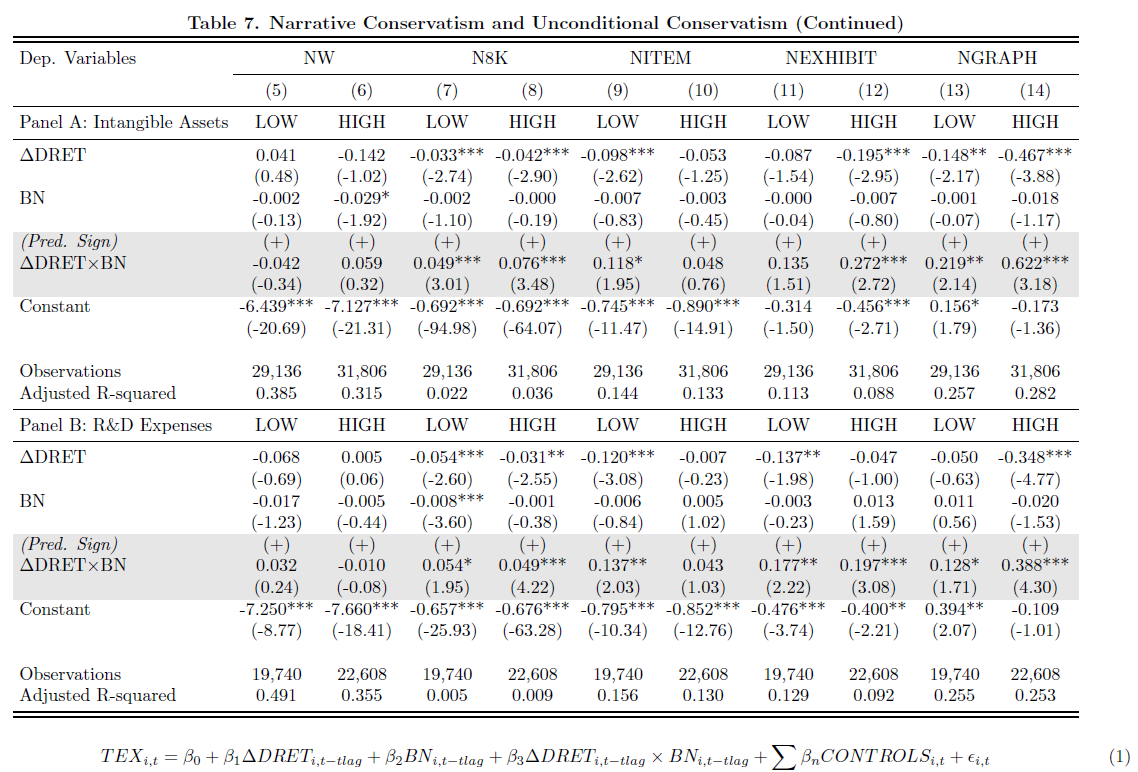
\includegraphics[width=0.8\linewidth]{tab7_cont}
		\label{tab7_cont}
	\end{figure}
	
\end{frame}
%------------------------------------------------
%\begin{frame}
%	\frametitle{Additional Analyses: Firm Characteristics}
%	\begin{figure}[h]
%		\centering
%		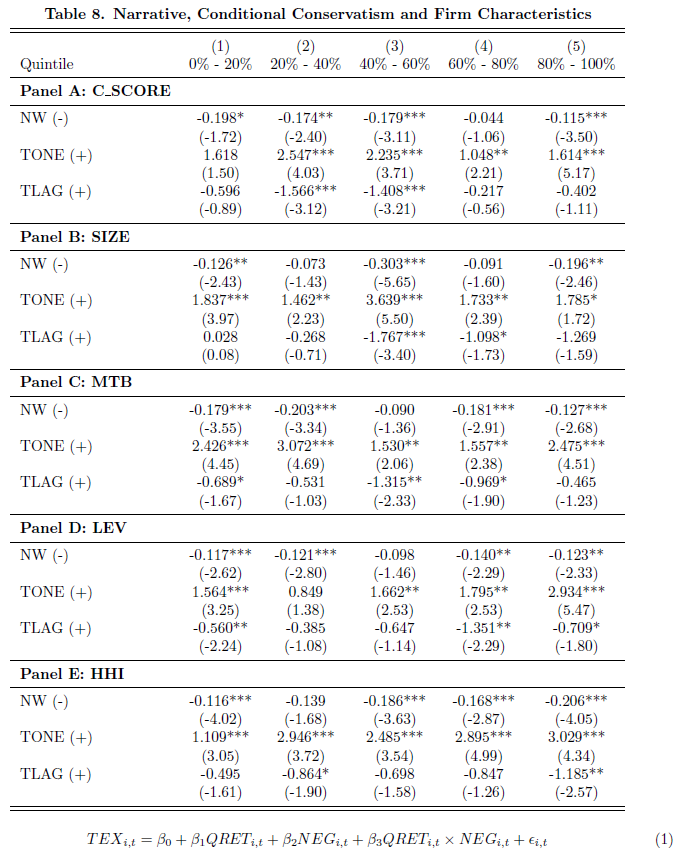
\includegraphics[width=0.5\linewidth]{tab8}
%		\label{tab8}
%	\end{figure}
%	
%\end{frame}
%%------------------------------------------------
%\begin{frame}
%	\frametitle{Additional Analyses: Managerial Incentives}
%	\begin{figure}[h]
%	\centering
%	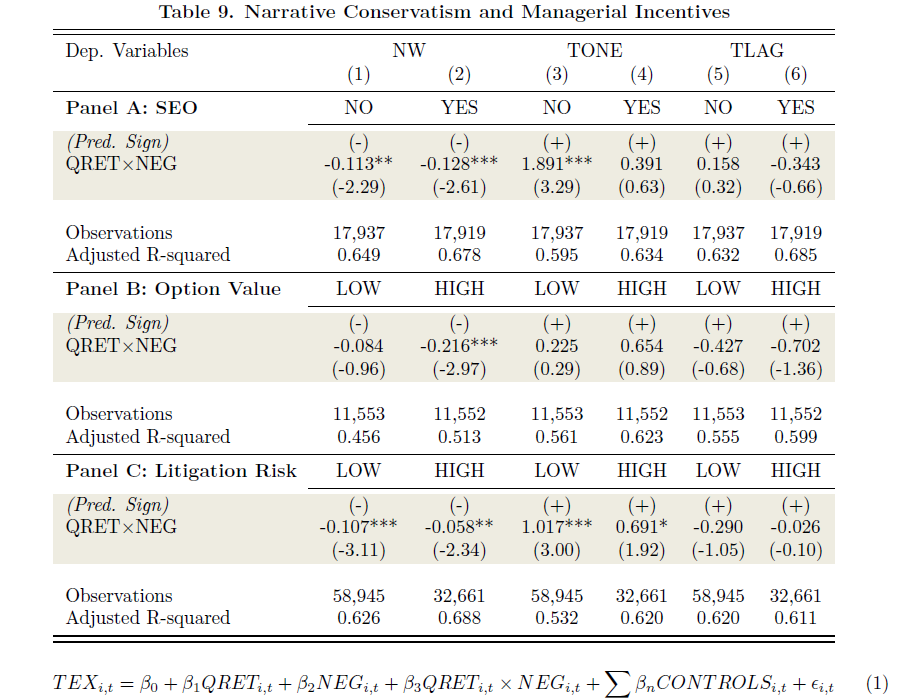
\includegraphics[width=0.7\linewidth]{tab9}
%	\label{tab9}
%	\end{figure}
%\end{frame}
%------------------------------------------------
\section{Conclusions}
%------------------------------------------------
\begin{frame}
\frametitle{Conclusions}
\begin{itemize}
	\item \textbf{Conclusions}
	\begin{itemize}
		\item We provide evidence that narratives reflect bad news in a more complete, news-consistent, and timely manner than good news. 
		\item Firms report lengthier 10-Qs to clarify rather than obfuscate bad news, and provide more 8-Ks and 8-K items in response to bad news than to good news.
		\item We document greater narrative conservatism in the MD\&A section and in voluntary disclosure. Also, narrative conservatism is pervasive in firms with high conditional conservatism, intangible assets, R\&D expenses and proprietary costs.
		\item We find greater narrative conservatism in settings where managers have strong incentives to disclose bad news.
	\end{itemize}

%	\item \textbf{Future Research}
%	\begin{itemize}
%		\item An aggregate measure of narrative conservatism
%		\item Economic implications of narrative conservatism
%		\item Mechanisms that assure the credibility of narrative conservatism 
%	\end{itemize}
	
\end{itemize}

\end{frame}
%------------------------------------------------
\section{References}
%------------------------------------------------
\beginbackup
\begin{frame}<presentation:0>
\frametitle{Selected References}
\scriptsize
\bibliographystyle{plainnat}
\bibliography{NC_slides}
\end{frame}
\backupend
%------------------------------------------------
\end{document}